\documentclass[12pt, a4paper]{article}

% Paquetes esenciales para el reporte
\usepackage[utf8]{inputenc}
\usepackage[spanish]{babel}
\usepackage{graphicx}
\usepackage{float}
\usepackage{amsmath}
\usepackage{amssymb}
\usepackage[T1]{fontenc}
\usepackage{booktabs} % Para tablas bonitas
\usepackage{fancyhdr} % Para encabezados y pies de página
\usepackage{lastpage} % Para obtener el número total de páginas
\usepackage{geometry} % Para configurar los márgenes
\usepackage{hyperref} % Para links y metadatos
\usepackage{longtable} % Para tablas que se extienden a varias páginas
\usepackage{tabularx} % Para tablas con ancho fijo
\usepackage{multirow} % Para combinar celdas
\usepackage{tikz} % Para los logos en la portada

% Configuración de márgenes
\geometry{a4paper, margin=2cm}

% Configuración de la paginación y el estilo de la página
\pagestyle{fancy}
\fancyhead{} % Borrar encabezado
\fancyfoot[C]{\thepage\ de \pageref{LastPage}} % Paginación en el centro del pie de página
\renewcommand{\headrulewidth}{0pt} % Sin línea en el encabezado
\renewcommand{\footrulewidth}{0.4pt} % Línea en el pie de página

% --- PORTADA ---
\begin{document}

% Para la portada sin paginación
\pagestyle{empty}

% Logos en las esquinas superiores
\begin{tikzpicture}[remember picture,overlay]
    % Logo UTM en la esquina superior izquierda
    \node[anchor=north west, inner sep=1cm] at (current page.north west)
        {\includegraphics[width=0.2\textwidth]{utm_logo.jpg}};
    % Logo de Ingeniería en Computación en la esquina superior derecha
    \node[anchor=north east, inner sep=1cm] at (current page.north east)
        {\includegraphics[width=0.18\textwidth]{compu_logo.jpg}};
\end{tikzpicture}

\begin{center}
    \vspace*{3cm} % Espacio vertical para centrar el contenido
    \Large\textbf{UNIVERSIDAD TECNOLÓGICA DE LA MIXTECA}
    
    \vspace{0.5cm}
    
    \vspace{1.5cm}
    \begin{Huge}\textbf{Proyecto: Análisis Financiero y Estadístico de Samsung Electronics}\end{Huge}
    
    \vspace{2.5cm}
    \begin{tabular}{l l}
    \textbf{Materia:} & Probabilidad y Estadística \\[0.8cm]
    \textbf{Profesor:} & Dr. Guillermo Arturo Lancho Romero \\[0.8cm]
    \textbf{Alumno:} & Pérez Cortes José Alberto \\[0.8cm]
    \textbf{Carrera:} & Ingeniería en Computación \\[0.8cm]
    \textbf{Semestre:} & Séptimo Semestre \\[0.8cm]
    \textbf{Grupo:} & 702-A \\
    \end{tabular}
    
    \vspace{3cm}
    \large\textbf{\today}
\end{center}

\newpage
\pagenumbering{arabic}
\setcounter{page}{1}

% --- INTRODUCCIÓN Y CONTEXTO DE LA EMPRESA ---
\section*{Introducción y Contexto de la Empresa}
\addcontentsline{toc}{section}{Introducción y Contexto de la Empresa}

\begin{center}
    
\includegraphics[width=0.25\textwidth]{samsung_logo.png} % Ajusta el ancho según el tamaño que quieras
\end{center}

\subsection*{Breve descripción de Samsung Electronics}
Samsung Electronics es una de las corporaciones multinacionales de tecnología más grandes y rentables del mundo, con sede en Suwon, Corea del Sur. Como la principal filial del Grupo Samsung, la empresa se dedica a una amplia gama de productos y servicios tecnológicos. Su negocio principal se divide en tres áreas principales:
\begin{itemize}
    \item \textbf{Consumer Electronics (CE):} Abarca productos para el hogar como televisores (donde es el líder mundial en ventas desde hace años), electrodomésticos (refrigeradores, lavadoras) y dispositivos de audio y video.
    \item \textbf{IT \& Mobile Communications (IM):} Incluye su famoso portafolio de teléfonos inteligentes Samsung Galaxy, tablets, laptops, dispositivos portátiles y soluciones de red para empresas. Desde 2012, Samsung ha sido el mayor fabricante de teléfonos inteligentes del mundo.
    \item \textbf{Device Solutions (DS):} Se enfoca en la fabricación de componentes electrónicos cruciales, como semiconductores (memorias DRAM y Flash), procesadores y pantallas (LCD, OLED) que no solo utiliza en sus propios productos, sino que también vende a otras grandes compañías de tecnología a nivel global.
\end{itemize}
A lo largo de los últimos años, Samsung ha mantenido una posición de liderazgo en múltiples mercados, lo que se refleja en sus fluctuaciones bursátiles y la alta variabilidad que a menudo muestra su precio en la bolsa.

\newpage

% --- CONTENIDO PRINCIPAL DEL REPORTE ---
\section{Análisis de la Evolución de Precios de Samsung}
\addcontentsline{toc}{section}{Análisis de la Evolución de Precios de Samsung}

\subsection*{Primeros y Últimos Datos}
A continuación, se presentan los precios de cierre diarios de Samsung Electronics para los primeros y últimos cinco días del período analizado (últimos 3 años), mostrados en las tres monedas principales: won surcoreano (KRW), dólares estadounidenses (USD) y pesos mexicanos (MXN). Estos datos nos dan un vistazo inicial a la tendencia general de la empresa en el tiempo.

\begin{figure}[H]
    \centering
    \begin{tabularx}{\textwidth}{@{}llll@{}}
        \toprule
        \multicolumn{4}{l}{\textbf{Primeros 5 Precios (en las tres monedas)}} \\
        \midrule
        \textbf{Fecha} & \textbf{Precio KRW} & \textbf{Precio USD} & \textbf{Precio MXN} \\
        \midrule
        2022-09-23 & 54,500 & \$41.92 & \$754.62 \\
        2022-09-26 & 53,900 & \$41.46 & \$746.31 \\
        2022-09-27 & 54,200 & \$41.69 & \$750.46 \\
        2022-09-28 & 52,900 & \$40.69 & \$732.46 \\
        2022-09-29 & 52,600 & \$40.46 & \$728.31 \\
        \bottomrule
    \end{tabularx}
    \par\vspace{1em}
    \begin{tabularx}{\textwidth}{@{}llll@{}}
        \toprule
        \multicolumn{4}{l}{\textbf{Últimos 5 Precios (en las tres monedas)}} \\
        \midrule
        \textbf{Fecha} & \textbf{Precio KRW} & \textbf{Precio USD} & \textbf{Precio MXN} \\
        \midrule
        2025-09-12 & 75,400 & \$58.00 & \$1,044.00 \\
        2025-09-15 & 76,500 & \$58.85 & \$1,059.23 \\
        2025-09-16 & 79,400 & \$61.08 & \$1,099.38 \\
        2025-09-17 & 78,200 & \$60.15 & \$1,082.77 \\
        2025-09-18 & 80,300 & \$61.77 & \$1,111.85 \\
        \bottomrule
    \end{tabularx}
    \caption{Precios de Cierre de Samsung (Primeros y Últimos 5 Días) en KRW, USD y MXN.}
    \label{tab:precios_cierre}
\end{figure}

\subsection*{Análisis de Tendencia y Variabilidad}
Los siguientes gráficos ilustran la evolución del precio de cierre de la acción de Samsung en los últimos 3 años, mostrados en las tres monedas principales. Las líneas azul, coral y verde muestran el precio diario en won surcoreano, dólares estadounidenses y pesos mexicanos, respectivamente. Las líneas de color naranja y rojo representan los promedios móviles de 30 y 90 días. La proximidad y el cruce de estas líneas indican la variabilidad del precio, mientras que su dirección general señala la tendencia (alta si el precio final es mayor que el inicial, o baja si es lo contrario).

\begin{figure}[H]
    \centering
    % Asegúrate de que las gráficas se guardaron en archivos .png o .pdf
    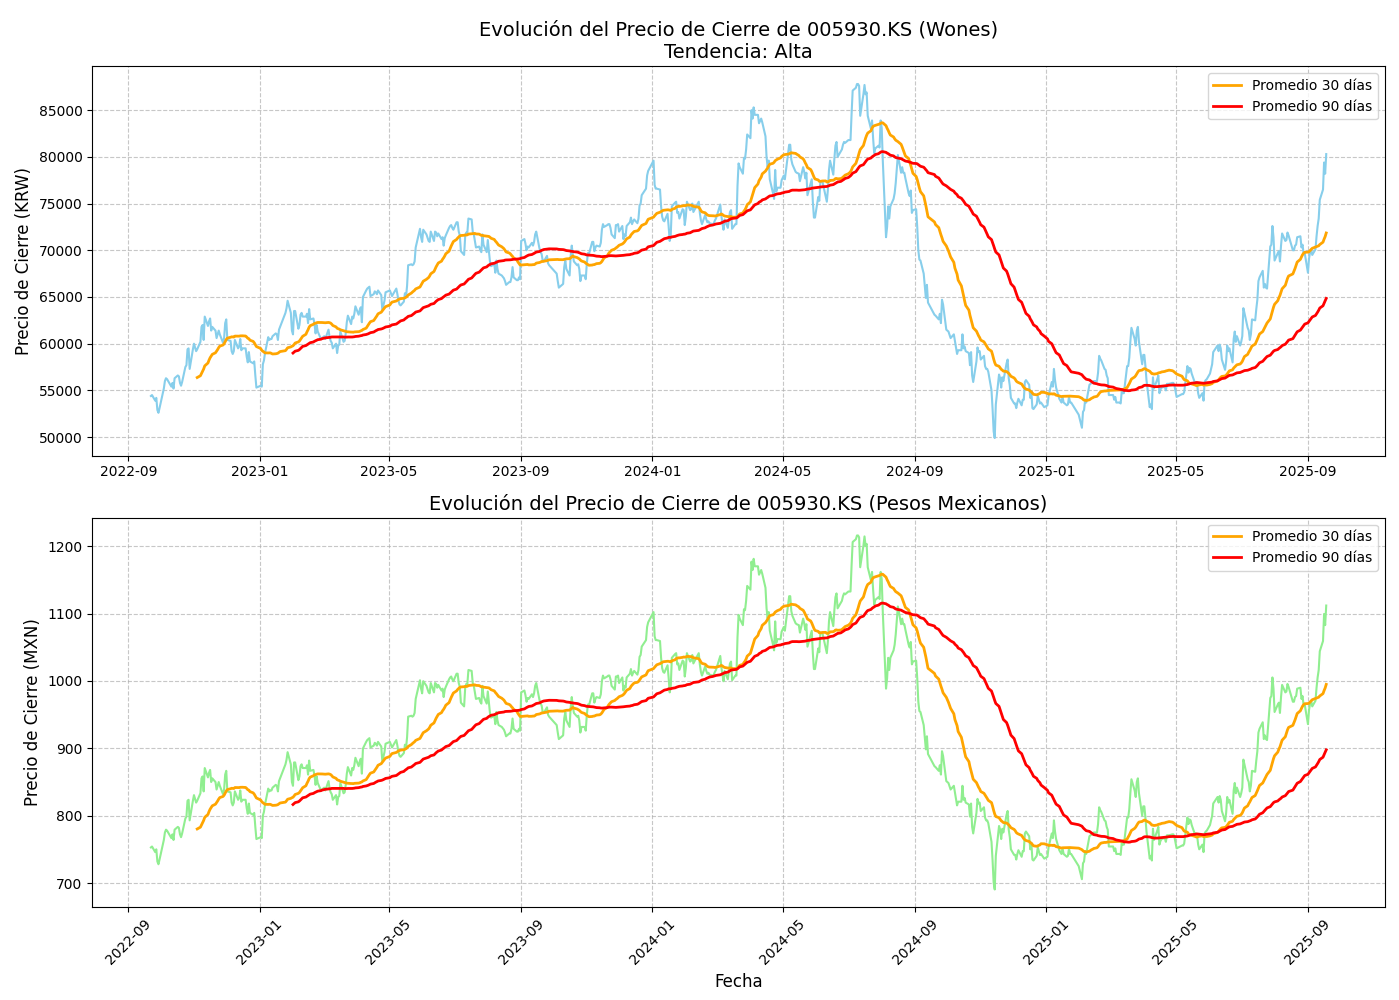
\includegraphics[width=\textwidth]{grafica_precio_evolucion.png}
    \caption{Gráfico de Evolución de Precios de Cierre de Samsung en las 3 Monedas (KRW, USD y MXN). La línea de tendencia general indica una tendencia alcista, a pesar de las fluctuaciones.}
    \label{fig:precio_evolucion}
\end{figure}

\newpage
\subsection*{Análisis de Rendimientos Logarítmicos}
Los rendimientos logarítmicos son una métrica crucial para analizar el desempeño de un activo, ya que miden el cambio porcentual de precio de un día a otro y son aditivos en el tiempo. A continuación se presenta el rendimiento de los primeros y últimos 5 días del análisis.

\begin{figure}[H]
    \centering
    \begin{tabularx}{\textwidth}{@{}lll@{}}
        \toprule
        \multicolumn{3}{l}{\textbf{Primeros 5 Rendimientos Logarítmicos}} \\
        \midrule
        \textbf{Fecha} & \textbf{Rendimiento} & \\
        \midrule
        2022-09-26 & -0.011070 & (-1.11\%) \\
        2022-09-27 & 0.005550 & (+0.56\%) \\
        2022-09-28 & -0.024278 & (-2.43\%) \\
        2022-09-29 & -0.005687 & (-0.57\%) \\
        2022-09-30 & 0.009461 & (+0.95\%) \\
        \bottomrule
    \end{tabularx}
    \par\vspace{1em}
    \begin{tabularx}{\textwidth}{@{}lll@{}}
        \toprule
        \multicolumn{3}{l}{\textbf{Últimos 5 Rendimientos Logarítmicos}} \\
        \midrule
        \textbf{Fecha} & \textbf{Rendimiento} & \\
        \midrule
        2025-09-12 & 0.026883 & (+2.69\%) \\
        2025-09-15 & 0.014483 & (+1.45\%) \\
        2025-09-16 & 0.037208 & (+3.72\%) \\
        2025-09-17 & -0.015229 & (-1.52\%) \\
        2025-09-18 & 0.026500 & (+2.65\%) \\
        \bottomrule
    \end{tabularx}
    \caption{Rendimientos Logarítmicos de los Primeros y Últimos 5 Días del Análisis.}
    \label{tab:rendimientos}
\end{figure}

\newpage
\subsection*{Estadísticas de Precios y Rendimientos en las Tres Monedas}
Las siguientes tablas resumen las estadísticas clave calculadas a partir de los datos de precios de cierre y rendimientos logarítmicos. La desviación estándar es una medida de la volatilidad; una mayor desviación indica un mayor riesgo. Los datos actualizados muestran información de 732 días de análisis con 731 rendimientos calculados.

\begin{figure}[H]
    \centering
    \begin{tabularx}{\textwidth}{@{}lXXX@{}}
        \toprule
        \textbf{Estadística} & \textbf{Won (KRW)} & \textbf{Dólares (USD)} & \textbf{Pesos (MXN)} \\
        \midrule
        Número de datos & 732 & 732 & 732 \\
        Mínimo & 49,900 & \$38.38 & \$690.92 \\
        Máximo & 87,800 & \$67.54 & \$1,215.69 \\
        Promedio & 66,333 & \$51.03 & \$918.45 \\
        Desviación Estándar & 8,716 & \$6.70 & \$120.68 \\
        \bottomrule
    \end{tabularx}
    \caption{Tabla de Estadísticas de Precios de Samsung en las Tres Monedas.}
    \label{tab:estadisticas_precios}
\end{figure}

\begin{figure}[H]
    \centering
    \begin{tabularx}{\textwidth}{@{}lX@{}}
        \toprule
        \textbf{Estadística} & \textbf{Rendimientos Logarítmicos} \\
        \midrule
        Número de rendimientos & 731 \\
        Mínimo & -0.108716 (-10.87\%) \\
        Máximo & 0.069661 (+6.97\%) \\
        Promedio & 0.000530 (+0.05\%) \\
        Desviación Estándar & 0.017583 (+1.76\%) \\
        \bottomrule
    \end{tabularx}
    \caption{Tabla de Estadísticas de Rendimientos Logarítmicos de Samsung.}
    \label{tab:estadisticas_rendimientos}
\end{figure}

\subsection*{Visualización de Estadísticas Descriptivas}
La siguiente gráfica presenta las estadísticas descriptivas de precios en formato de barras, facilitando la comparación visual entre las diferentes métricas estadísticas. Se muestran el mínimo, máximo, media muestral, varianza (dividida entre 10,000 para mejor visualización) y desviación estándar en won surcoreano y dólares estadounidenses.

\begin{figure}[H]
    \centering
    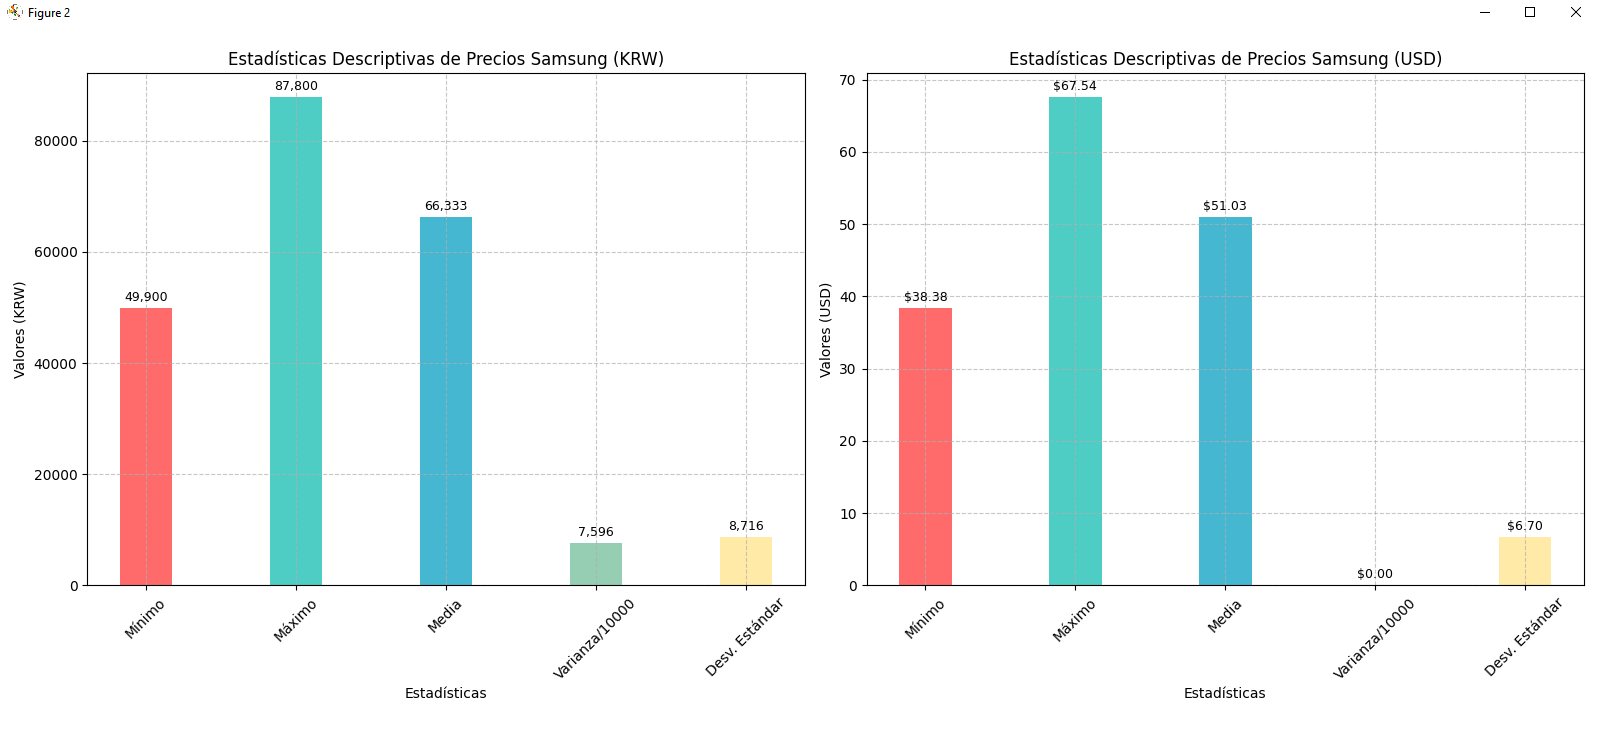
\includegraphics[width=\textwidth]{grafica_estadisticas_descriptivas.png}
    \caption{Gráfica de Barras de Estadísticas Descriptivas de Precios de Samsung en KRW y USD. Los valores numéricos facilitan la interpretación de las métricas estadísticas.}
    \label{fig:estadisticas_descriptivas}
\end{figure}

\subsection*{Evolución de Rendimientos en el Tiempo}
Esta gráfica muestra la evolución temporal de los rendimientos logarítmicos, permitiendo identificar períodos de alta y baja volatilidad. Las líneas horizontales representan la media y las desviaciones estándar (±1σ), mientras que los puntos rojos destacan los valores extremos (±2σ).

\begin{figure}[H]
    \centering
    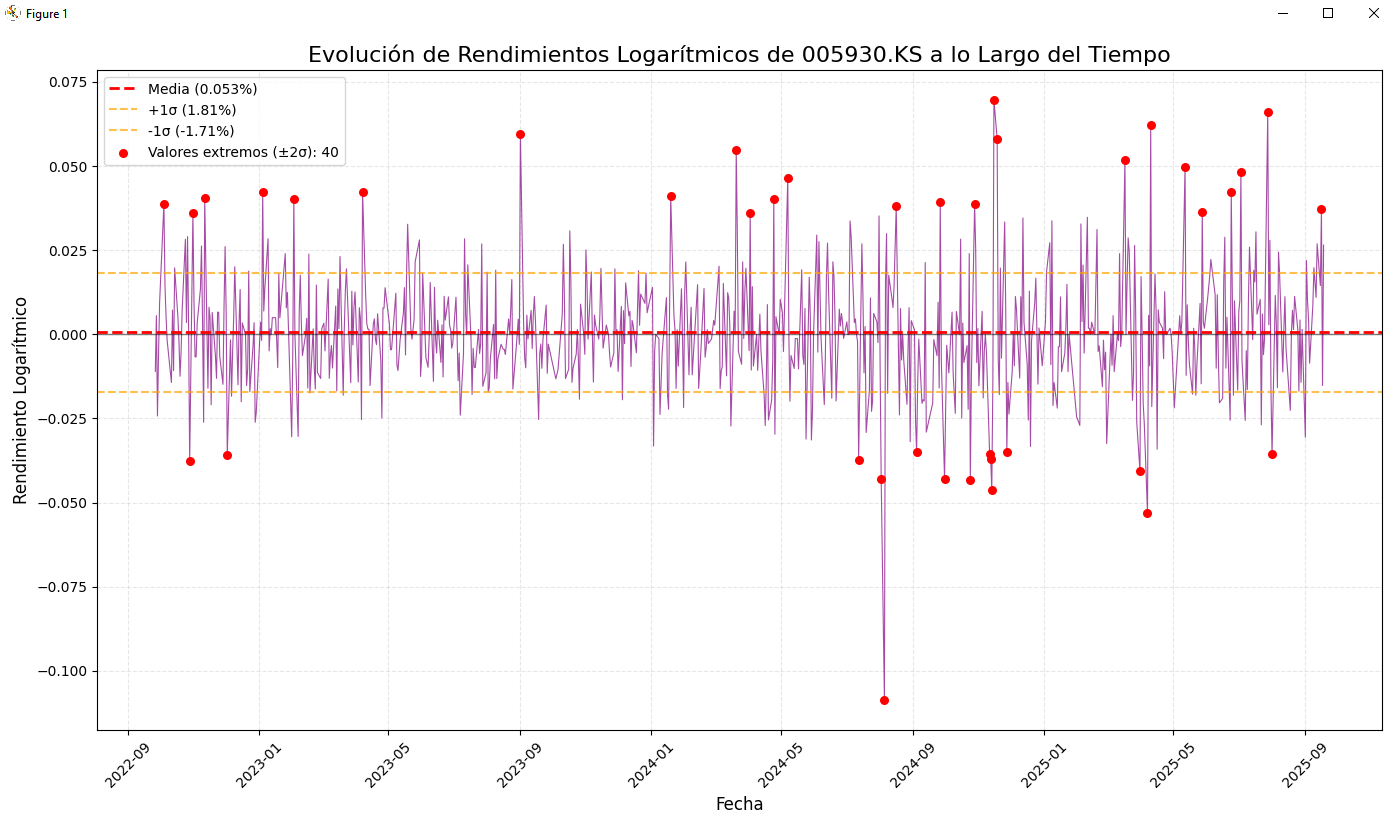
\includegraphics[width=\textwidth]{grafica_tiempo_rendimientos.png}
    \caption{Evolución Temporal de Rendimientos Logarítmicos de Samsung. Los valores extremos señalan eventos de alta volatilidad en el mercado.}
    \label{fig:tiempo_rendimientos}
\end{figure}

\subsection*{Distribución de los Rendimientos}
La gráfica de caja y bigotes es una herramienta útil para visualizar la distribución de los rendimientos de la acción. La caja central muestra el 50\% de los datos, la línea media es la mediana, y los puntos fuera de los "bigotes" representan valores atípicos (días con rendimientos extremadamente altos o bajos).

\begin{figure}[H]
    \centering
    % Asegúrate de que las gráficas se guardaron en archivos .png o .pdf
    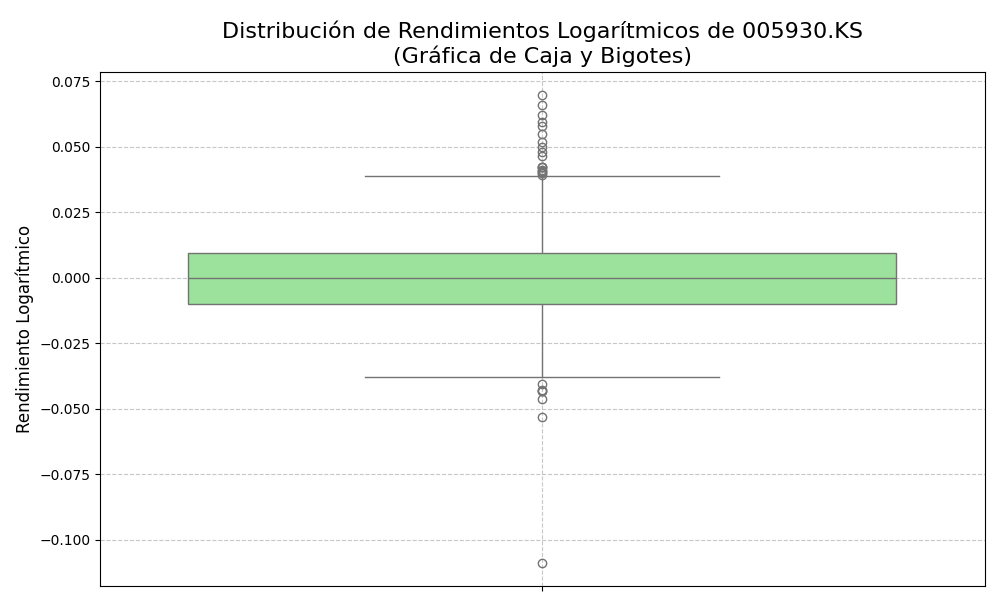
\includegraphics[width=0.8\textwidth]{grafica_caja_bigotes.png}
    \caption{Gráfico de Caja y Bigotes de Rendimientos Logarítmicos. La presencia de valores atípicos indica una alta volatilidad en algunos días.}
    \label{fig:caja_bigotes}
\end{figure}

\newpage
\subsection*{Comparación Detallada de Precios en las Tres Monedas}
Finalmente, esta tabla permite una comparación específica entre dos fechas seleccionadas, detallando el precio en las tres monedas, la diferencia absoluta y el cambio porcentual. El ejemplo mostrado corresponde a la comparación realizada entre el 27 de enero de 2023 y el 25 de septiembre de 2023, donde se observó un crecimiento del 7.43\%.

\begin{figure}[H]
    \centering
    \begin{tabularx}{\textwidth}{@{}l l l l@{}}
        \toprule
        \textbf{Métrica} & \textbf{Fecha 1} & \textbf{Fecha 2} & \textbf{Cambio} \\
        \midrule
        \textbf{Fecha} & 2023-01-27 & 2023-09-25 & - \\
        \textbf{Precio KRW} & 64,600 & 69,400 & +4,800 \\
        \textbf{Precio USD} & \$49.69 & \$53.38 & +\$3.69 \\
        \textbf{Precio MXN} & \$894.46 & \$960.92 & +\$66.46 \\
        \textbf{Cambio \%} & - & - & +7.43\% \\
        \bottomrule
    \end{tabularx}
    \caption{Comparación Detallada de Precios entre dos Fechas Seleccionadas en las Tres Monedas.}
    \label{tab:comparacion_detallada}
\end{figure}

\subsection*{Tipos de Cambio Utilizados}
Para las conversiones monetarias realizadas en este análisis, se utilizaron los siguientes tipos de cambio aproximados:
\begin{itemize}
    \item \textbf{1 USD = 1,300.00 KRW} (Won surcoreano)
    \item \textbf{1 USD = 18.00 MXN} (Peso mexicano)
    \item \textbf{1,000 KRW = \$0.77 USD = \$13.85 MXN}
\end{itemize}

Estos tipos de cambio fueron obtenidos automáticamente por el sistema, pero debido a problemas de conectividad, se utilizaron valores aproximados para mantener la consistencia del análisis.

\end{document}